\section{Analyzing the Component Electrical Models}
\subsection{Charged Disc Embedded in Dielectric: A Point Charge-like Electric Field}\label{cpt:charged disc}
\hspace{0em}\indent Consider a disc of radius $R=1$, charged with $q$, embedded in a semi-infinite dielectric. let $\theta_s$ be the arc of the disc in contact with the dielectric.

The dielectric structure is symmetric about $\theta_s$, which corresponds to the right angle at the contact point in Figure \ref{fig:disk in D}. However, it allows for variation in how much the disc is embedded, as measured by the parameter $\theta_s$.
\begin{figure}[H]
    \centering
    \adjustbox{frame=0.25pt,frame,margin=0.15pt,color=mycolor}{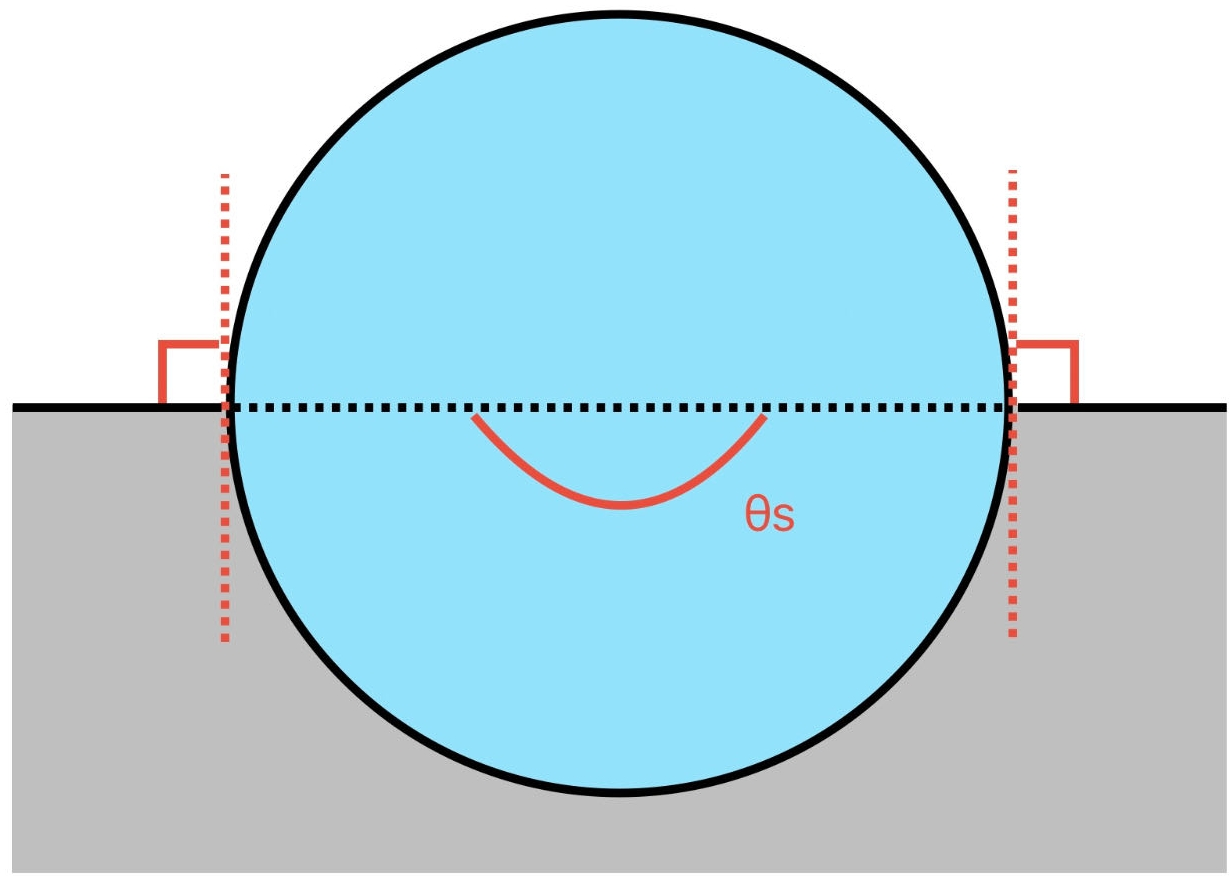
\includegraphics[width=0.46\linewidth]{Figs/sketch disk embedded right.jpg}}\hfill
    \adjustbox{frame=0.25pt,frame,margin=0.15pt,color=mycolor}{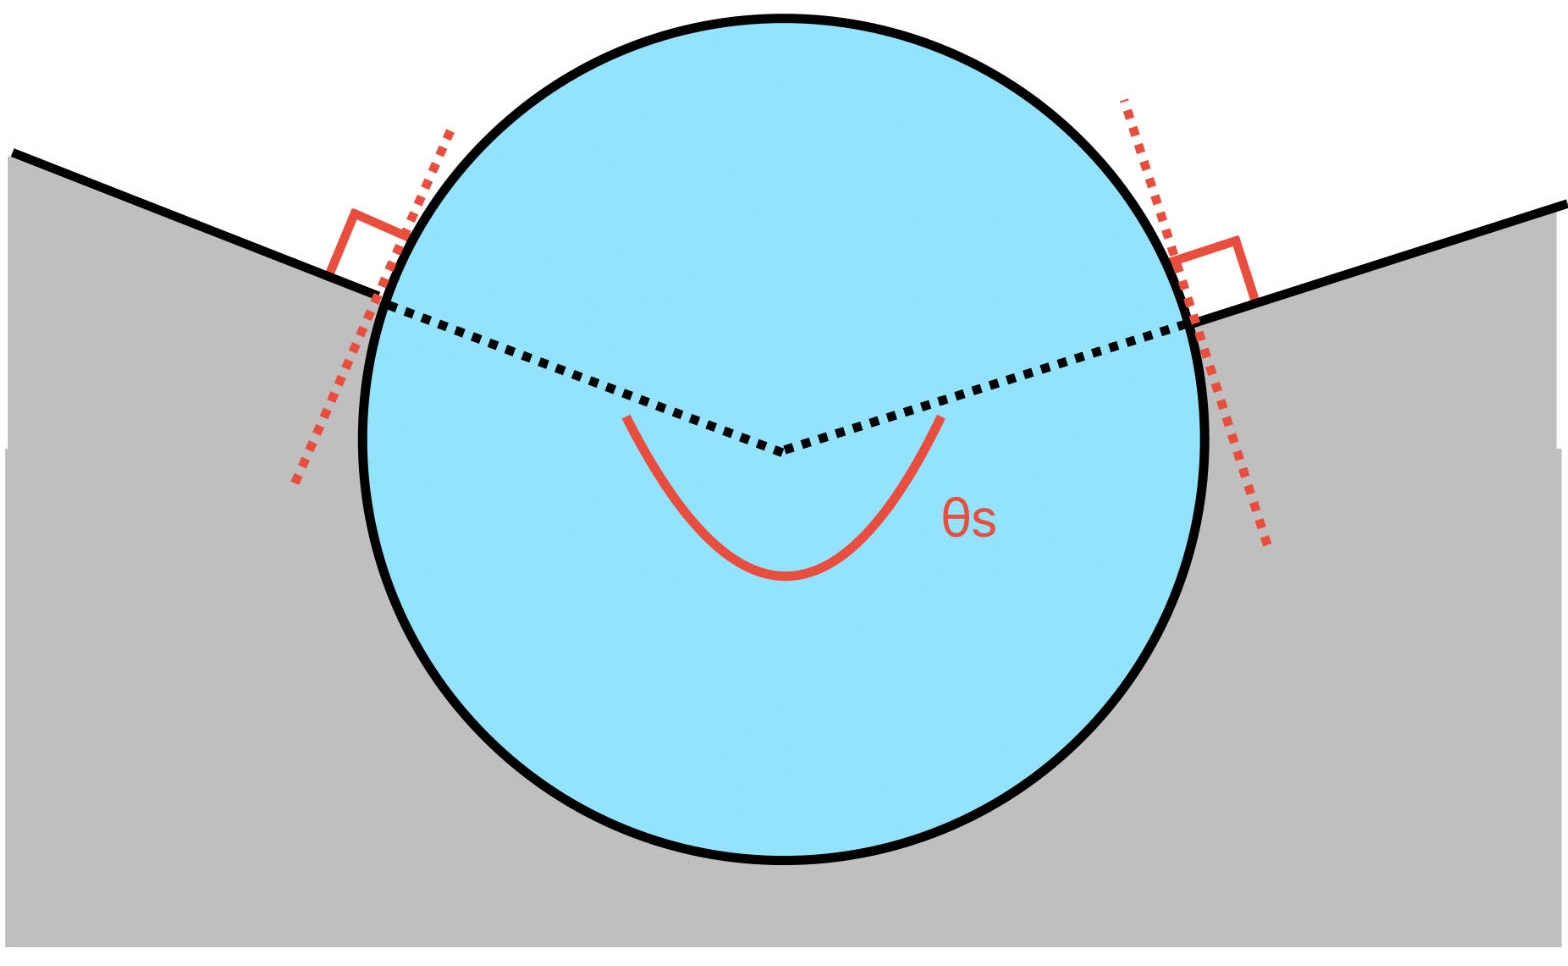
\includegraphics[width=0.531\linewidth]{Figs/sketch disk embedded angle.jpg}} % Side by side images
    
    \caption{\small Two cases are presented where the disc is embedded in a dielectric, measured by $\theta_s$. The left figure shows the case where $\theta_s=\pi$, while the right figure depicts a different $\theta_s$. It is found that the electric fields of the cases differ based on $\theta_s$.}
    \label{fig:disk in D}
\end{figure}

Postulate that the far-field voltage is 
\[V_{\infty}=  \frac{q'}{2\pi\epsilon_0} \log r\]
where $q'\not\equiv q$ is some magnitude of charge. If the voltage satisfies the necessary local boundary conditions, we can be confident that this is the correct voltage for the configuration according to the uniqueness theorem (\ref{uniqueness}).

On the boundary between the droplet and the dielectric, $R=1, \theta\in(0\footnote{Let the point where the dielectric contacts the disc from the left be the zero angle.}, \theta_s)$. According to equation (\ref{eqn:die surf q}),
\[
\sigma_b = \vec{P}\cdot\hat{n}=\epsilon_0 \chi_e E_{\hat{r}}
\]
where\footnote{Note that along the arc, the normal direction of the dielectric boundary points toward the origin. Let the disc be positively charged; the electric field of the disc points outward. Also, note that the sum of the induced surface charge (from both the dielectric and the disc) is positive, with its own electric field lines pointing outward, which is why there are two minus signs in equation (\ref{eqn:surf dq}). }
\begin{equation}\label{eqn:surf dq}
    E_{\hat{r}} = -E_{q} - \frac{\sigma_b}{2 \epsilon_0}  
\end{equation}
Hence
\[
\sigma_b= \epsilon_0 \chi_e \left( -\frac{q}{2 \pi R \epsilon_0} - \frac{\sigma_b}{2 \epsilon_0} \right)
\Longrightarrow \sigma_b = -\frac{q}{2 \pi R} \cdot \frac{2 \chi_e}{2 + \chi_e}
\]
Postulate that the surface charge density in the dielectric\footnote{At the contact line of the dielectric and the disc, the total surface charge density is the sum of both.} on the arc at $R=1$ is uniformly $\sigma_b$, then the total surface charge $q_s$ is
\[\sigma_b \int^{\theta_s} R\df\theta= -q \frac{2 \chi_e}{2 + \chi_e}\cdot\frac{\theta_s}{2 \pi} =q_s\]
let $\theta_s=\pi$ in our case, the total charge $q_t$ of the system is then
\begin{equation}\label{eqn:disk,d,qt}
    q_t=q+q_s=q(1-\frac{1}{2}\frac{2\chi_e}{2+\chi_e})=q\frac{2}{2+\chi_e}\leq q
\end{equation}
The electric field is unique everywhere, regardless of whether it is in the dielectric or not:
\[
\vec{E}=\frac{q_t}{2\pi\epsilon_0 r}\hat{r}=\frac{q}{2\pi\epsilon_0 r}\frac{2}{2+\chi_e}\hat{r}
\]
and the voltage is:
\[
v=\frac{1}{2\pi\epsilon_0}\frac{2q}{2+\chi_e}\log r
\]
The electric field is symmetric about the origin; its field lines parallel to the dielectric boundary along $\pm x$. Hence, the dielectric contains no surface charge other than $\sigma_b$ on the arc.

The surface charge distribution on the disc, $\sigma_d$, is then
\begin{align*}
\sigma_d&= \begin{cases}q_t/\pi &, \theta\in(0,\pi) \\
|\sigma_b| + q_t/\pi &,  \theta\in(\pi,2\pi)\end{cases}
\end{align*}

\subsection{Point Charge Embedded in Dielectric: Different Electric Fields in Various Regions}\label{cpt:charge in die}
\hspace{0em}\indent For a point charge embedded in a dielectric below the $x$-axis, the three types of charges in this setup are the free charge, the induced volume charge, and the induced surface charge.

The free charge $q_f$ is simply the point charge $q$. The point charge induces a volume charge density $\rho_b$ at $\vec{r}_0(x,y) = (0, -d)$, \[q_b=\int_\mathcal{V}\rho_b\Longleftrightarrow \rho_b = q_b\delta(\vec{r}-\vec{r}_0)
\]
and an induced surface charge density $\sigma_b$.

The two quantities need to be determined to satisfy the following boundary conditions, equation (\ref{eqn:v.cts}), which ensures continuity in voltage, and equation (\ref{eqn:gauss}), which applies Gauss's Law to the surface charge density.

The electric field consists of two different components. For the voltage inside the dielectric, we treat the charge and the induced volume charge field as a single entity $q$, Gauss's Law provides:
\[
V = \frac{q}{2\pi\epsilon} \log(r - r_0)
\]
where $\epsilon$ is the permittivity.

By method of Image, we replace the dielectric with induced charges and treat all charges as if they were in a vacuum, using $\epsilon_0$, hence 
\[V_{q}=\frac{q}{2\pi\epsilon_0} \log(r-r_0)\]
and
\[V_{q_b}=\frac{q_b}{2\pi\epsilon_0} \log(r-r_0)\]
By equation (\ref{eqn:P}), $\vec{P}=\epsilon\chi_e \vec{E}$, and equation (\ref{eqn:rho_b}), $\rho_b\coloneqq-\nabla\cdot\vec{P}$,
\[q_b\coloneqq\int_{\mathcal{V}} \rho_b\delta (\vec{r}-\vec{r}_0)=-\frac{\chi_e}{1+\chi_e}q\Longrightarrow q+q_b=\frac{1}{1+\chi_e}q=\frac{q}{\epsilon_r}
\]
the two voltages sum to
\[
V=V_q+V_{q_b}=\frac{1}{2\pi\epsilon_0}\frac{q}{\epsilon_r}\log (r-r_0)=\frac{1}{2\pi\epsilon_0}\frac{q}{\epsilon_r}\log\sqrt{(x-0)^2+(y--d)^2}
\]
the electric field pointing $\hat{y}$ is
\[
E_y=-\frac{\partial V}{\partial y}=\frac{1}{2\pi\epsilon}\frac{q}{\sqrt{(x)^2+(y+d)^2}}\frac{1}{\sqrt{(x)^2+(y+d)^2}}\frac{1}{2}2(y+d)=\frac{1}{2\pi\epsilon}\frac{q(y+d)}{x^2+(y+d)^2}
\]
at $y=0$
\[
E_q=\frac{1}{2\pi\epsilon}\frac{qd}{x^2+d^2}=\frac{1}{2\pi\epsilon_0}\frac{1}{1+\chi_e}\frac{qd}{x^2+d^2}
\]
by equation (\ref{eqn:ed.line}), surface charge density satisfies
\[
E_\sigma=-\frac{\sigma_b}{2\epsilon_0}
\]
and by equation (\ref{eqn:rho_b}), $\sigma_b=\vec{P}\cdot\hat{n}=\epsilon_0\chi_e\vec{E}\cdot\hat{n}$, from the two we find
    \[    \sigma_b=\epsilon_0\chi_e\left(E_q+E_{\sigma}\right)=\epsilon_0\chi_e\left(\frac{1}{2\pi\epsilon_0}\frac{1}{1+\chi_e}\frac{qd}{x^2+d^2}-\frac{\sigma_b}{2\epsilon_0}\right)\Longrightarrow
        \frac{2+\chi_e}{2}\sigma_b=\frac{1}{2\pi}\frac{\chi_e}{1+\chi_e}\frac{qd}{x^2+d^2}
    \]
hence the induced surface charge density of the dielectric, on $y=0$, is
\[
\sigma_b=q\frac{\chi_e}{1+\chi_e}\frac{1}{2+\chi_e}\frac{ d / \pi}{x^2+d^2}
\]
\subsection{Dielectric Shielding and the Difference from \citeauthor{Griffiths_2017}}\label{cpt:shield}
\hspace{0em}\indent After deriving the electric properties for the models above, we find that our results are inconsistent with similar cases in Chapter 4 of \citet{Griffiths_2017}. In Example 4.5 on page 187, the textbook derives the case of a metal sphere charged $Q$, surrounded by dielectric of finite radius and finds that in the region $\vec{r}>\vec{r}_{\mathcal{D}}$,
\[E_{textbook}\sim Q/\epsilon_0\] 
However, using our derivation method, the electric field is found to be
\[E= \frac{1}{4 \pi r^2}\frac{Q}{\epsilon_0}\frac{2}{2+\chi_e}\] 
which is smaller by a factor $\frac{2}{2+\chi_e}$ compared to the textbook result. The other two similar cases from \citet{Griffiths_2017} are Problem 4.35, concerning a point charge in a spherical dielectric; and Problem 4.38, regarding a conducting sphere embedded in a dielectric\footnote{See \citet{Griffiths_2017}, Ex. 4.5, p. 187 and Problem 4.35, p. 206, for reference.}.

In these cases, the textbook derives without considering certain surface charge densities. All our results are smaller by a factor of $\frac{2}{2+\chi_e}$, and the details of calculations are omitted here.

Hence we need to examine carefully if they match the required local boundary conditions in our situation. For the point charge in the dielectric case, we check whether the integral of the surface charge density, $q_s$, cancels out the induced volume charge $q_b$
\[
q_s\coloneqq\int_S \sigma_b \df a \Longrightarrow \int_\mathbb{R}\sigma_b \df x=q\frac{1}{1+\chi_e}\frac{\chi_e}{2+\chi_e}\frac{d}{\pi}\int_\mathbb{R}\frac{1}{x^2+d^2}\df x=...\frac{d}{\pi} \frac{\pi}{d}=q\frac{\chi_e}{1+\chi_e}\frac{1}{2+\chi_e}
\]
Yet the amount of induced volume charge is:
\begin{equation}\label{eqn:sigma_b}
q_b=\int_\mathcal{V}-\nabla\cdot\vec{P}=-\nabla\cdot\epsilon_0\frac{\chi_e}{\epsilon}\vec{D}=- q\frac{\chi_e}{1+\chi_e}    
\end{equation}
we observe that $q_s \neq q_b$. If they were equal, it would almost imply that, when observed from the outside, the dielectric appears to have no effect\footnote{Which is the scenario presented in \citet{Griffiths_2017} examples, and is not in this thesis. The derivation follows.}. Since this is not the case, we must locate the surplus charge to determine the dielectric's actual effect in the situation. 

The voltage below is the potential due to three point charges. The charges $q_f$ and $q_b$ at $(x,y) = (0,-d)$, sum to
\[
q_r=q_f + q_b = (1-\frac{\chi_e}{1+\chi_e} )q =\frac{1}{1+\chi_e}q=\frac{q}{\epsilon_r}
\]
and the induced surface charge sums to $q_s$. We locate it at $(x,y)=(0,d)$. The voltage below the $x$-axis is therefore
\begin{align*}
    V_{below}&=\frac{1}{2\pi\epsilon_0}\left(q_r\log\sqrt{x^2+(y+d)^2} +q_s\log\sqrt{x^2+(y-d)^2}\right)
    \\&=\frac{q}{2\pi\epsilon_0}\left(\frac{1}{\epsilon_r}\log\sqrt{x^2+(y+d)^2} +\frac{\epsilon_r-1}{\epsilon_r}\frac{1}{\epsilon_r+1}\log\sqrt{x^2+(y-d)^2}\right)
    \\&=\frac{q}{2\pi\epsilon_0}\left(\frac{1}{\chi_e +1}\log\sqrt{x^2+(y+d)^2} +\frac{\chi_e}{1+\chi_e}\frac{1}{2+\chi_e}\log\sqrt{x^2+(y-d)^2}\right)    
    \\&=\frac{q}{2\pi\epsilon_0\epsilon_r}\left(\log\sqrt{x^2+(y+d)^2} +\frac{\chi_e}{2+\chi_e}\log\sqrt{x^2+(y-d)^2}\right)    
    \end{align*}

For the voltage above the $x$-axis, locate $q_s$ at $(x,y) = (0,-d)$, while the other two remain at their original positions. The three charges sum to
\[q_t=
q_o+q_b+q_s=\frac{q}{\epsilon_r}+\frac{q}{\epsilon_r}\frac{\chi_e}{2+\chi_e}=\frac{q}{1+\chi_e}\frac{2+2\chi_e}{2+\chi_e}=\frac{2q}{\chi_e+2}
\]
hence the voltage is
\[
V_{above}=\frac{1}{2\pi\epsilon_0}\frac{2 q}{({\chi_e+2})}\log\sqrt{x^2+(y+d)^2}=\frac{q}{\pi\epsilon_0}\frac{1}{(\epsilon_r+1)}\log\sqrt{x^2+(y+d)^2}
\]
Moreover, check if Gauss's Law satisfies
\begin{align*}
\frac{\partial V_{above}}{\partial y}-\frac{\partial V_{below}}{\partial y}&=\frac{q}{2\pi} \left( \frac{2}{\epsilon_r + 1} \frac{y + d}{x^2 + (y + d)^2} - \frac{1}{\epsilon_r} \frac{y + d}{x^2 + (y + d)^2} -\frac{1}{\epsilon_r} \frac{\epsilon_r-1}{\epsilon_r+1}\frac{y - d}{x^2 + (y - d)^2}\right)   
\end{align*}
at $y=0$
\begin{align*}
\left.\frac{\partial V_{upper}}{\partial y}-\frac{\partial V_{lower}}{\partial y}\right|_{y=0}&=\frac{q}{2\pi} \frac{d}{x^2 + d^2}\left( \frac{2}{\epsilon_r + 1} - \frac{1}{\epsilon_r} +\frac{1}{\epsilon_r}\frac{\epsilon_r-1}{\epsilon_r + 1}  \right) \\
    &=\frac{q}{2\pi}  \frac{d}{x^2 + d^2}  \frac{2\epsilon_r -\epsilon_r -1+\epsilon_r -1}{\epsilon_r(\epsilon_r + 1)} \\
    &=\frac{q}{2\pi}  \frac{d}{x^2 + d^2} \frac{2\epsilon_r -2}{\epsilon_r(\epsilon_r + 1)} \\
    &=\frac{q}{\pi}  \frac{d}{x^2 + d^2} \frac{\epsilon_r -1}{\epsilon_r(\epsilon_r + 1)}=\frac{q}{\pi}  \frac{d}{x^2 + d^2}\frac{\chi_e}{\chi_e +1}\frac{1}{\chi_e +2}
\end{align*}

It matches $\sigma_b$ in equation \ref{eqn:sigma_b}; Gauss's Law is fulfilled\footnote{For further confirmation, see a related problem at \citet{Griffiths_2017} Ex 4.25, p. 207.}. 

The voltage $V_{above}$ describes how the dielectric affects the surroundings. We observe that the apparent magnitude of the charge $q_s$ varies, yet it retains the form of a point charge with a fixed location. Consequently, the problem of the point charge, dielectric, and droplet reduces to that of a point charge field, differing only in the charge magnitude, which is advantageous.

Furthermore, an interesting phenomenon was observed: the voltage outside the dielectric is not as commonly expected, as though the dielectric had no effect at all:
\[
V_{expected}=\frac{q}{2\pi\epsilon_0}\log\sqrt{x^2+(y+d)^2}
\]
implies the dielectric leaves no effect on the external  region\footnote{If this were true, we receive two electric signals from the same charge, once sent from the vacuum, and once enclosed by dielectric before sending. There will be no difference between the two.}.  

Our derivation shows the quantity of a charge embedded in a dielectric, as seen from outside, is less than it actually is.
\[
\frac{V_{upper}}{V_{expected}}=\frac{q}{\pi\epsilon_0(\epsilon_r+1)} / \frac{q}{2\pi\epsilon_0}=\frac{2}{1+\chi_e+1}\leq 1\vspace{3em}
\]
Physically, this claims the dielectric shields some of the electric energy of embedded charges, which sounds plausible. The equipotentials of the point charge embedded in the dielectric are as follows.
\begin{figure}[H]
    \centering
    \adjustbox{frame=0.25pt,frame,margin=0.15,color=mycolor}{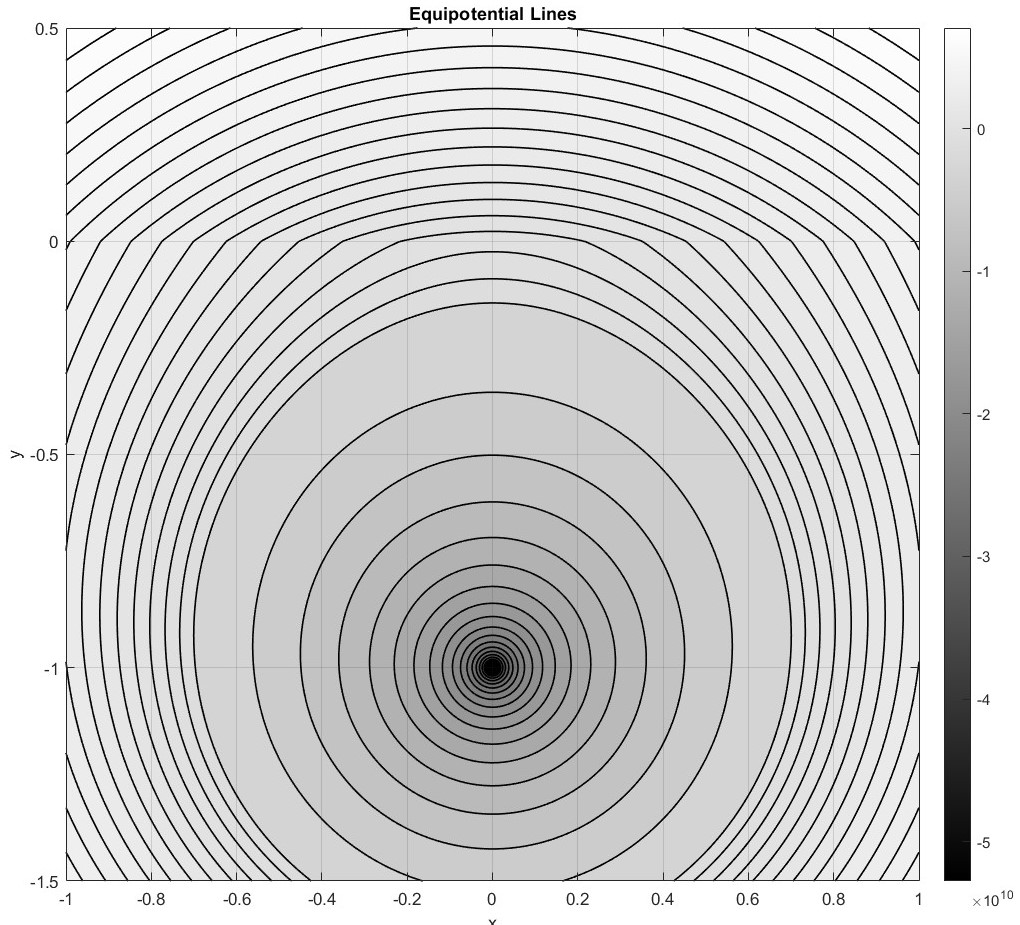
\includegraphics[width=1.\linewidth]{Figs/dieletic potential.jpg}}
    \caption{\small The equipotentials of a point charge embedded in the dielectric exhibit a noticeable change in direction at \(y=0\), which is the boundary between the dielectric and the air above. This indicates that the electric field is disrupted while the potential remains continuous due to the induced surface charge. In the region \(y>0\), the potential forms concentric circular equipotential lines created by a charge located at \(y=-d\), which has a smaller magnitude than the actual charge.
 }
    \label{fig:enter-label}
\end{figure}

In the case of a charged disc embedded in a dielectric, we find that $q_t\leq q$ in equation (\ref{eqn:disk,d,qt}), which also demonstrates the shielding effect.